\color{Blue}
\section{Algorithms}
An \colorbox{Yellow}{algorithm} is a \textbf{systematic} and \textbf{unambiguous} procedure producing an answer to a question/a solution in \colorbox{Yellow}{finite} \textbf{number of steps}.
\\ Algorithm has an input, sometimes, input needs to satisfy conditions. Algorithm has output (usually solution).
\\ \colorbox{Yellow}{Good algorithms} consist of correctness, speed, space \& simplicity. 
\\ Correctness: right answer/right answer most of the time/close to right answer
\\ Space: Amount of mem needed
\\ Simplicity: easy to understand, analyze, implement, debug, modify, update
\paragraph{Iterative algorithms} Problem solved by iterating (step-by-step), often using loops.
\paragraph{In-place algorithms} Uses constant amount of memory (in addition of that used to store input). Important, because if data barely fits mem, don't want an algo using twice memory to sort.
\\ Selection and Insertion in-place, just swapping. MergeSort is \textcolor{Red}{not} in-place, merge needs temporary array.
\\ QuickSort can easily be made in-place
\subsection{Binary Search}$O(\log{n})$ Search for if something is in a list, like using a dictionary, split in half and check if lower or upper, then check corresponding half.\\ %\textbf{$n \log(n)$} comparisons\\
\textbf{In} array of n elements, a \textbf{key} k to search for \textbf{Out} array sorted in increasing order
\begin{algorithmic}
\State binarySearch(a,n,k)
\State left $\to$ 0
\State right $\to$ n
\While{$right>left+1$} 
	\State mid $\gets$ $\lceil (left+right)/2 \rceil $
	\If{$A[mid]>k$} right $\gets$ mid 
	
	\Else left $\gets$ mid
	\EndIf
\EndWhile
\If{$A[left]=k$} return True;
\Else return False;
\EndIf
\end{algorithmic}
\subsection{Bubble Sort} $O(n^2)$
\\ Sort \# in ascending. Loop through list many times, if 2 elem next to each other wrong order, swap (need tmp var). ct is count, last N-2-ct elements already sorted on pass.
\begin{algorithmic}
	\For{$ct\gets 1$ to $N-2$}
		\For{$i\gets 0$ to $N-2-ct$}
			\If{$list[i]>list[i+1]$}
				\State swap($list[i],list[i+1]$)
			\EndIf
		\EndFor
	\EndFor
\end{algorithmic}
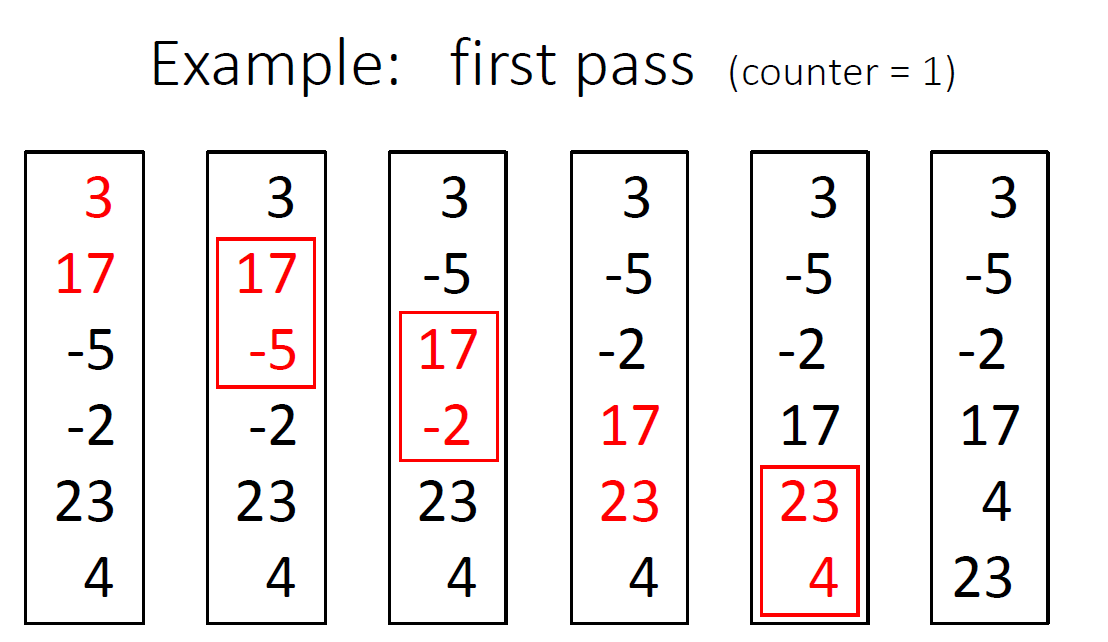
\includegraphics[scale=0.13]{bs}
\subsection{Selection Sort} $O(n^2)$
\\ Sort \# in ascending. Partition list into 2, sorted and remain. Find smallest from remain and add to sorted and so on. (\colorbox{Yellow}{SWAP})
\begin{algorithmic}
\For{$i \gets 0$ to $N-2$}
	\State $tmpIndex \gets i$
	\\//{i is first element in rest}
	\State $tmpMinValue \gets list[i]$
	\For{$k=i+1$ to $N-1$}
		\If{$list[k]<tmpMinValue$}
			\State $tmpIndex\gets k$
			\State $tmpMinValue\gets list[k]$
		\EndIf
	\EndFor
	\If{$tmpIndex != i$}
		\State swap($list[i],list[tmpIndex]$)
	\EndIf
\EndFor
\end{algorithmic}
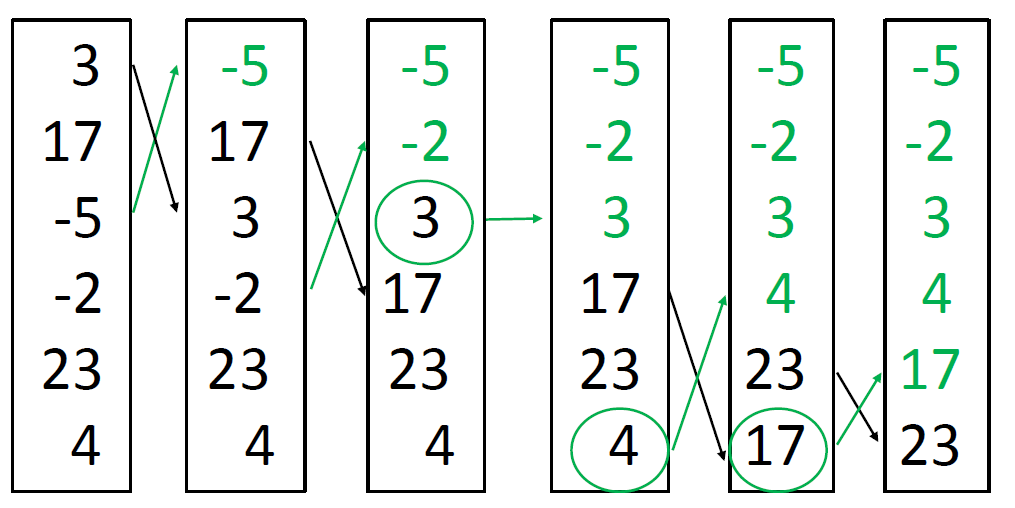
\includegraphics[scale=0.13]{ss}
\subsection{Insertion Sort} $O(n^2)$ for worst, $O(n)$ for best. Insert index k into correct position wrt 0 to k-1. i.e. 0 to k-1 already sorted, insert k at proper position
\begin{algorithmic}
	\For{$k \gets 1$ to $N-1$}
		\State $elementK \gets list[k]$ // Store kth element, will overwrite
		\State $i \gets k$
		\While{$i>0$ and $list[i-1]>elementK$} // $i>0$ first to avoid out of bound
			\\//{Shift everything bigger than kth to the right to fit k}
			\State $list[i] \gets list[i-1]$
			\State $i \gets i-1$
		\EndWhile
		\State $list[i] \gets elementK$
	\EndFor 
\end{algorithmic}
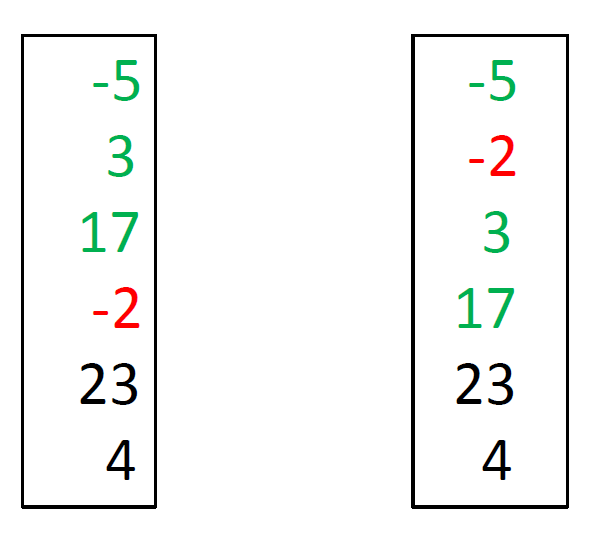
\includegraphics[scale=0.1]{is}\\
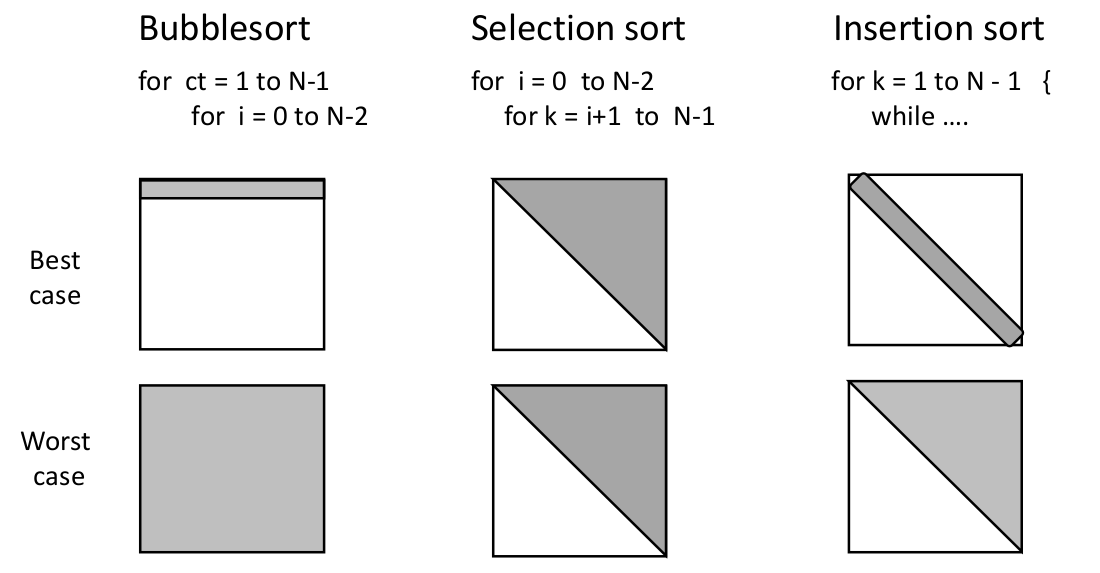
\includegraphics[scale=0.13]{sort3}
\\------------------
\section{Multiplication Algorithms}
\paragraph{Iterative}, add $b$, $a$ times.
\paragraph{Standard} Grade school multiplication.\\
$a=a_0a_1\ldots a_{k-1},b=b_0b_1\ldots b_{n-1}$
\begin{algorithmic}
	\State $total \gets 0$
	\For{$i \gets n-1$ to $0$}
		\State $carry \gets 0$
		\State $tmpAdd \gets$ Array of $k+1$ digits
		\For{$j \gets k-1$ downto $0$}
			\State $c\gets b_i*a_j+carry$
			\State $tmpAdd_{j+1}\gets c \mod 10$
			\State $carry \gets \lfloor c/10 \rfloor$
		\EndFor
		\State $tmpAdd_0 \gets carry$
		\State $total \gets total+tmpAdd*10^{(n-i-1)}$
	\EndFor
	\State return total
\end{algorithmic}
\paragraph{Recursive} Split into 2 halves, $a=10^{\lfloor k/2 \rfloor }l_a+r_a,b=10^{\lfloor n/2 \rfloor }l_b+r_b$.
\\$ab=(10^{\lfloor k/2 \rfloor}l_a+r_a)(10^{\lfloor n/2 \rfloor }l_b+r_b)=r_a r_b+10^{\lfloor n/2 \rfloor}r_al_b+10^{\lfloor k/s \rfloor}l_ar_b+10^{\lfloor k/2 \rfloor + \lfloor n/2 \rfloor }l_al_b$
\\ Implement recursively, base case is single digit mult, if statements for $n>1$ and $k>1$ for term1, $k>1$ for term2, $n>1$ for term3.
%\begin{algorithmic}
%	\If{$k=1$ and $n=1$} return $a_0 *b_0$
%	\EndIf
%	\State $term1 \gets term2 \gets term3 \gets term3 \gets 0$
%	\State $l_a \gets (a_0\ldots a_{k-\lfloor k/2 \rfloor -1})$
%	\State $r_a \gets (a_{k-\lfloor k/2 \rfloor }\ldots a_k-1)$
%	\State $l_b \gets (b_0\ldots b_{n-\lfloor n/2 \rfloor -1})$
%	\State $r_b \gets (b_{n-\lfloor n/2 \rfloor -1})$
%	\If
%\end{algorithmic}
\paragraph{Recursive Fast} Same as recursive, but combine term3 and 4 into 1 multiplication.
\\$(l_a+r_a)*(10^{\lfloor n/2 \rfloor - \lfloor k/2 \rfloor l_b+r_b}l_b+r_b)=10^{\lfloor n/2 \rfloor - \lfloor k/2 \rfloor}l_al_b+(l_ar_b+10^{\lfloor n/2 \rfloor - \lfloor k/2 \rfloor}l_b+r_b)-10^{\lfloor n/2 \rfloor - \lfloor k/2 \rfloor}l_al_b-r_ar_b$
\\ This is term3, and so we get:
\\$a*b=10^{\lfloor k/2 \rfloor + \lfloor n/2 \rfloor}term2+10^{\lfloor k/2 \rfloor}term3+term1$
\color{Fuchsia}
\section{\textcolor{Fuchsia}{Recursion}}
Algo is recursive if, while solving prob, calls itself 1+ times. Need a \colorbox{Yellow}{base case} so recursion \textcolor{Red}{stops}. Examples:
\subsection{Recursive power computation}
\begin{algorithmic}
	\State \textbf{Algorithm} power(a,n)
	\If{n=0} return 1
	\Else 
		\State $previous \gets power(a,n-1)$
		\State return $previous*a$
	\EndIf
\end{algorithmic}
\subsection{Binary Search} Can implement through recursion. In: sorted array, start, stop, key. Out: index found or -1 if not found. Split in half, then recall binary search with corresponding half (depending on whether current index is larger or smaller than key) to check. \colorbox{Yellow}{Base case} is when start=stop, check if value is key, else false.
\subsection{Fibonacci Sequence} $F(0)=0, F(1)=1 \& F(n)=F(n-1)+F(n-2)$ if $n\geq 2$
\paragraph{\colorbox{Red}{Iterative}}
\begin{algorithmic}
	\If{$n=0$} return 0
	\EndIf
	\If{$n=1$} return 1
	\EndIf
	\State $previous \gets 0$
	\State $current \gets 1$
	\For{$i=2$ to $n$}
		\State $tmpCurrent \gets current$
		\State $current \gets current+previous$
		\State $previous \gets tmpCurrent$
	\EndFor
	\State return current
\end{algorithmic}
\paragraph{Recursive} although still \textcolor{Red}{not efficient}.
$O(2^n)$
\begin{algorithmic}
	\If{$n=0$} return 0
	\ElsIf{$n=1$} return 1
	\Else return Fib(n-1)+Fib(n-2)
	\EndIf
\end{algorithmic}
\color {CarnationPink}
\section{\textcolor{CarnationPink}{Divide-and-Conquer}} Many recursive algorithms: 
\textbf{Divide} prob into subprob, \textbf{conquer} subprob by solving them recursively, \textbf{combine} the subsols
\subsection{MergeSort}$O(n log n)$ Array to be sorted, divide in 2 halves, conquer by recursively sorting each half, then merge each half
\\ To merge, create temp array with left and right indices, constantly comparing
\\ Given 2 sorted halves, merge to one sorted array. left to mid sorted, mid+1 to right sorted.
\begin{algorithmic}
\State \textbf{Algorithm} merge(A, left, mid, right)
\State $indexLeft \gets left$ //Left half index
\State $indexRight \gets mid+1$ //Right half
\State $tmp \gets $ Array of same type and size as A
\State $tmpIndex \gets left$ // start at begin
\While{$tmpIndex \leq right$} // Go up to right
	\If{$indexRight > right$ or ($indexLeft \leq mid$ and $A[indexLeft]\leq A[indexRight]$)} //indexRight is end or indexLeft isn't at mid yet and element there is smaller than at indRight (left smaller than right)
		\State $tmp[tmpIndex] \gets A[indexLeft]$ // Take left \& increment
		\State $indexLeft \gets indexLeft+1$
	\Else //Right isn't at end, right is smaller than left
		\State $tmp[tmpIndex]\gets A[indexRight]$ // Take right
		\State $indexRight \gets indexRight+1$
	\EndIf
	\State $tmpIndex \gets tmpIndex+1$
\EndWhile
\For{$k \gets left$ to $right$} $A[k] \gets tmp[k]$ // Copy tmp to A
\EndFor
\end{algorithmic}
mergeSort, keep splitting in half until you merge trivial, recursion
\begin{algorithmic}
	\State \textbf{Algorithm} mergeSort (A, left, right)
	\If{$left<right$} // At least 2 elements
		\State $mid \gets \lfloor (left+right)/2 \rfloor $
		\State mergeSort($A,left,mid$)
		\State mergeSort($A,mid+1, right$)
		\State merge($A,left,mid,right$)
	\EndIf
\end{algorithmic}
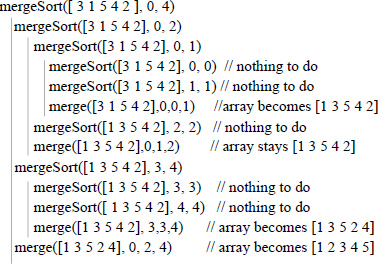
\includegraphics[scale=0.4]{ms}\\
Something like $T(n)=1+2T(n/2)+n$
\subsection{QuickSort}
$O(n^2)$, but usually faster than MergeSort, since $O(n log n)$ on average. Not as reliable because of $n^2$. Divided and conquer again. Pick a \colorbox{Yellow}{pivot} and put smaller things on left, bigger on right, then insert pivot in middle and use recursion.
\begin{algorithmic}
	\State \textbf{Algorithm} quickSort(A,start,stop)
	\If{$start<stop$} 
		\State $pivotIndex \gets partition(A,start,stop)$
		\State quickSort($A,start,pivotIndex-1$)
		\State quickSort($A,pivotIndex+1,stop$)
	\EndIf
\end{algorithmic}
Worst case is when already sorted. Usually will split into roughly equal parts if random. Easier to do in-place than MergeSort.
\\ partition, takes an array with indices and stop, out: return index j, rearranges all elements of A so all indexes below j are lower than A[j] and all above are greater than A[k]
\\ $A = [6, 3, 5, 9, 2, 5, 7, 8, 4, \tikz \node[draw,circle]{5};_{\text{pivot}}]$
\\ $\stackrel{\text{partition}}{\rightarrow} \underbrace{3,5,2,5,4}_{\leq pivot}, 5_{\text{pivot}}\underbrace{6,9,7,8}_{\geq pivot}$
\\ Quicksort each side now
\\$ 3,5,2,5,\tikz\node[draw,circle]{4};_{pivot}$\hspace{20 pt} $6,9,7,\tikz\node[draw,circle]{8};_{pivot}$
\\ $\stackrel{\text{partition}}{\rightarrow}\underbrace{3,2}_{\leq pivot}, 4 ,\underbrace{5,5}_{\geq pivot}$ \hspace{20 pt} $\underbrace{6,7}_{QS},8,\underbrace{9}_{QS}$
\\ Quicksort again
\\ $2,3,4,5,5,5,6,7,8,9$
\begin{algorithmic}
	\State \textbf{Algorithm} partition(A,start,stop)
	\State $pivot \gets A[stop]$
	\State $left \gets start$
	\State $right \gets stop-1$
	\While{$left < right $}
		\While{$left < right$ and $A[left]<pivot$} $left \gets left+1$
		\EndWhile
		\While{$left < right$ and $A[right]\geq pivot$} $right \gets right-1$
		\EndWhile
		\\ //Basically keep indexing left and right until number on left and right don't belong, swap
		\If{$left<right$} exchange $A[left]\leftrightarrow A[right]$
		\EndIf
	\EndWhile
	\State exchange $A[stop]\leftrightarrow A[left]$
	\State return left
\end{algorithmic}
\color{Orange}
\section{\textcolor{Orange}{Loop invariants}}
Algo can be described by input, output, \textbf{preconditions} (restrictions on input), \textbf{postconditions}
\\ Ex: Bin search, input, array of integers, output index, prec: array sorted in ascending, postc: index is in array, -1 if not
\\ Check \colorbox{Green}{correctness} of algo: for correct input data, \textbf{stops} and produces correct output, input satisfies prec, output satisfies postc. How to prove? 
\\ \colorbox{Green}{Loop Invariant} loop property that holds before and after each iter of loop. To prove using LI, need 3 things:
\\ \textbf{Initialization:} true before first iter of loop, \textbf{maintenance:} true before an iter and stays true before next iter, \textbf{termination} when loop terminates, invariant gives useful prop to show correct
\\ Similar to induction, \textbf{base case}, \textbf{inductive step}. Invariant holds before first iter (base case), invariant holds from iter to iter (inductive step), termination is different, stops induction. Can show 3 in any order.
\paragraph{Example}Insertion sort
\\ Loop invariant: A[0...i-1] sorted. \textbf{Init} before i=1, A[0] sorted, \textbf{Maint} inserting ith element keeps A sorted \textbf{Term} outer for loop ends when i is length of A. Plug into i-1, get A[0...length-1], which is same as original Array, but sorted
\paragraph{FindMin} In: array A of n int, Out: smallest
\begin{algorithmic}
	\State Algo FindMin($A,n$)
	\State $i \gets 1$
	\State $m \gets A[0]$
	\While{$i<n$}
		\If{$A[i]<m$} $m\gets A[i]$
		\State $i \gets i+1$
		\EndIf
	\EndWhile
	\State return m
\end{algorithmic}
LI here is: at iter i, $m=min\{A[0],\ldots,A[i-1]\}$
\\init: $i=1,m=A[0]=min\{A[0]\}$
\\maint: Assume LI holds at begin, $m=min\{A[0],\ldots,A[i-1]\}$
\\2 conditions, $A[i]<m$: replace $A[i]$ makes $m=min\{\ldots A[i]\}$
\\ $A[i]\geq m$, then don't change m and $m=min\{\ldots A[i]\}$
\\ term: Algo will stop because i will reach n. Loop stops when $i=n$, so by LI, $m=min\{A[0],\ldots,A[n-1]\}$
\color{ForestGreen}
\section{\textcolor{ForestGreen}{Running time}}
Measure \colorbox{Yellow}{speed} of algo. But, depends on \textbf{size} of input, so describe as \colorbox{Yellow}{function} of input size.
\\ Also depends on \textbf{content} of input, like, if sorted or not
\\ 3 possibilities, best case (usually meaningless), average case (hard to measure), \colorbox{Yellow}{worst case} (good for safety critical \& easier to estimate)
\section{Primitive Operations} Ops that can be performed in constant time, assume they all take same time
\\$T_{assign},T_{call},T_{return},T_{arith},T_{comp}$ (compare)$,T_{cond},T_{index},T_{ref}$(follow obj ref)
\\ To find func of running time, add all primitives, including things depending on n (loops)
\color{Gray}
\section{\textcolor{Gray}{Big-O}} Simplify discussion of runtime, describe how running time is for LARGE n, grows as most fast as $O(g(n))$
\\ $f(n)$ and $g(n)$ 2 non-negative funcs defined on $\mathbb{N}$
%\begin{equation*}
	$f(n) \text{ is } O(g(n)) \iff \exists n_0\in \mathbb{N}, \exists c \in \mathbb{R}, st. \forall n\geq n_0, f(n) \leq c\cdot g(n)$
%\end{equation*}
c \textcolor{red}{cannot} depend on n
\\ To \colorbox{Yellow}{prove} $f(n)$ is $O(g(n))$, find $n_0$ and $c$ to satisfy conditions. Manipulate inequalities.
\\ To \colorbox{Yellow}{prove} $f(n)$ is \textcolor{Red}{not} $O(g(n))$, show for any $n_0$ and $c$, there's an $n\geq n_0$ st. $f(n)>c g(n)$ (usually n is in terms of c)
\subsection{Hierarchy}
%\begin{equation*}
	$O(1)\subset O(\log{n}) \subset O(\sqrt{n}) \subset O(n) \subset O(n^k) \subset O(2^n)$
	\\$O(1)$, functions bounded above by a constant.
%\end{equation*}
\subsection{Shortcuts}
\textbf{1. Sum rule.} $f_1(n)\in O(g(n))$ \& $f_2(n)\in O(g(n))$ then $f_1(n)+f_2(n)\in O(g(n))$ Can prove using 2 cs and 2 ns
\\\textbf{2. Constant factors rule} $f(n)\in O(g(n))$ then $kf(n)\in O(g(n))$ for any constant $k$. 
\\\textbf{3. Product rule} $d(n)\in O(f(n))$ and $e(n)\in O(g(n))$ then $d(n)\cdot e(n)\in O(f(n)\cdot g(n))$
\\ 4. $n^x \in O(a^n)$ for fixed $x>0$ and $a>1$
\\ 5. $log(n^x)\in O(log(n))$ for fixed $x>0$. Prove by $log(n^x)=x log(n)$
\\ 6. $\log_a(n)\in O(\log_b(n))$, prove by dividing, $\log_a(n)=\log_b(n)/\log_b(a)$
\paragraph{Limits}
1. $\lim_{n\to +\infty}f(n)/g(n)=0\implies f(n)\in O(g(n)) \& g(n)\notin O(f(n))$
\\2. $\lim_{n\to +\infty}f(n)/g(n)=x\neq 0\implies f(n)\in O(g(n)) \& g(n)\in O(f(n))$
\\3. $\lim_{n\to +\infty}f(n)/g(n)=+\infty \implies g(n)\in O(f(n)) \& f(n)\notin O(g(n))$
\\4. $\lim_{n\to +\infty}f(n)/g(n)$ does not exist, says nothing
\\ Remember l'H\^opital's rule: $\lim_{n\to +\infty} f(n)/g(n)=\lim_{n\to +\infty} \frac{df(n)/dn}{dg(n)/dn}$
\subsection{Big-Theta}
$f(n)$ is $\Theta(g(n)) \iff f(n)$ is $O(g(n))$ and $g(n)$ is $\Theta(f(n))$
\subsection{Big-Omega}
$f(n)$ is $\Omega(g(n)) \iff g(n)$ is $O(f(n))$
\color{RoyalBlue}
\section{\textcolor{RoyalBlue}{Abstract Data Types}}
Model of a data structure that specifies type of data stored and operations supported on data. Specifies what \colorbox{Yellow}{can be done} with data, but \textcolor{Red}{not} how it is done. Implementation of ADT specifies how operations are performed. User does not need to know about implementation.
\subsection{List ADT} Stores an ordered set of objects of any kind. 
\\Operations: \textbf{getFirst() :} returns first obj, \textbf{getLast():} returns last object of list, \textbf{getNth(n):} returns n-th obj, \textbf{insertFirst(Obj o)} : adds o at begin, \textbf{insertLast(obj o)}: adds o the end of the list,\textbf{ insertNth(n,o)} : adds n-th object as o,\textbf{ removeFirst()}: remove first obj, \textbf{removeLast()}: remove last o, \textbf{removeNth(n)}, \textbf{getSize()}: returns \# of obj in list, \textbf{concatenate(List I)}: append I to end of this list
\\ Implementation with an \colorbox{Green}{Array}
\\ 1D array L to store elements, int size for \# obj stored (\textcolor{Red}{not} capacity)
\\ getFirst() will return L[0], getLast() returns L[size-1] and getNth(n) returns L[n]
\\ insertLast increments size and puts at last spot, but insertNth has to shift all elements by 1 and increment
\\removeLast decrease size by 1 (no need to del things)
\\removeNth shifts over nth, size-1
\\ Arrays \textcolor{Green}{good} sine easy to implement \& space efficient
\\ \textcolor{Red}{Limitations}, size has to be known in advance, mem needed might be larger than num of elem used, insert or del can take $O(n)$. Array implementation is bad when \# of objects not known in advance and/or lots of insertions or removals.
\\ Implementation with a \colorbox{Green}{linked-list}, sequence of nodes, store data and which node is next in list. Have \textbf{head} and \textbf{tail}. \colorbox{Green}{recursive} data structure.
\\ \textcolor{Green}{Good} since don't need to know size, can expand and shrink easy, memory proportional to size
\begin{lstlisting}[language=java]
public class node{
private Object value;
private node next;
//Constructor	
public node
(Object x, node n){
	value=x;
	next=n;}
public node getNext(){
return next;}
public Object getValue(){
return value;}
public void 
setValue(Object x){
value=x;}
public void setNext(node n){
next=n;}
}

class linkedList{
node head,tail;
//default constr, empty list
list(){
	head=null;
	tail=null;}
getFirst(){
if(head==null) throw..
return head.getValue();}
getLast(){
if(tail==null) throw..
return tail.getValue();}
getNth(){
// throws outofbounds if...
node current=head;
while(n>0){
current=current.getNext();
n--;}
return current;}
void addLast(Object x){
if(tail==null){//empty list
tail=head=new node(x,null);}
else{
tail.setNext(new node(x,null));
tail=tail.getNext();}
}
void addFirst(Object x){
// less costly than Array
// O(1) here vs O(n)
head=new node(x,head);
if(tail==null) tai=head;}
insertNth(int n, Object x){
// throw if out of bounds
while(n>1){
predecessor=
predecessor.getNext();
n--;}
node newelem=
new node(x,predecessor.getNext());
predecessor.setNext(newelem);
return true;}
removeFirst(){
if(head==null){
return false;}
head=head.getNext();}
removeLast(){
if (tail==null){
return false;}
tmp=head.getNext();
while(tmp.getNext!=tail)
tmp=tmp.getNext}
tail=tmp;
tail.setNext(null);}
remove(Object x)
//throw if not found
if(head==null) //throw empty
if(head.getValue().equals(x)){
head=head.getNext();
if(head==null)tail=null;
return true;}
node current=head;
while(current.getNext()!=null &&
!current.getNext().
getValue().equals(x))
// right before x{
current=current.getNext();}
if(current.getNext()==
null) return false;
else{
current.setNext(current.getNext().
getNext());
if(current.getNext()==null){
tail=current;}
} return true;
}
\end{lstlisting}
\subsection{Stacks} ADT list only allowing ops at one end of list (top) 
\paragraph{Ops} \textbf{push(obj)}:insert elm at top, \textbf{obj pop()}; removes obj at top; \textbf{obj top()}: return last inserted w/o remove, peek() in java, \textbf{size()}: \# elem, boolean \textbf{isEmpty()}: empty?
\\ Stack is a Last in - First out (LIFO)
\\ Use: browser history, undo, chain of method calls in JVM
\\ Method Stack in JVM consists of every method call, with local vars and return, etc. Allows recursion
\paragraph{Array-based Stack}
\begin{lstlisting}[language=java]
public class ArrayStack{
	private Object S[];
	private int top=-1;
	public ArrayStack
	(int capacity){
	S=new Object[capacity]}
}
\end{lstlisting}
index t keeps track of top element
\begin{algorithmic}
	\State push(o)
	\If{$t=S.length-1$}
		\State throw FullStackEx
	\Else
	\State $t\gets t+1$
	\State $S[t] \gets o$
	\EndIf
	\State size()
	\State return $t+1$
	\State pop()
	\If{isEmpty()}
		\State throw EmptyEx
	\Else $t \gets t-1$
	\EndIf
\end{algorithmic}
Perf: $O(n)$ space, ops take $O(1)$. Limits: Need max size, push into full gives exception
\\ Can use Singly Linked List instead
\\ top element is stored first node
\\ Space used $O(n)$ and each operation takes $O(1)$
\\ Can use stacks to check if parenthesis match, put opening bracket on stack and remove if it finds a match, valid if stack is empty at end
\subsection{Queues} First in first out data structure, first come first serve service
\paragraph{Ops} void\textbf{ enqueue(obj o)}: add o to read, obj \textbf{dequeue()}: remove obj at front, exc if not, obj \textbf{front()}: returns obj at front, doesn't remove, exc if empty, int\textbf{ size()}: return \#, boolean \textbf{isEmpty()}:empty?
\\ Implement with linked-list
\\enqueue>addLast; dequeue>removeFirst; front>getFirst; empty>empty; size>size
\\ All $O(1)$ \textcolor{Red}{except} size $O(n)$
\paragraph{Double-ended queues} deque, allows insertion+removal from front and back
\\ Implement with linked list:
\\ getFirst(),getLast(); addFirst(o);addLast(o); isEmpty(); removeFirst(); all $O(1)$
\\removeLast(); size(); $O(n)$
\\\textcolor{Red}{Problem}: removeLast takes $O(n)$
\\ To do it faster: doubly-linked-list, have ref to prev too
\begin{lstlisting}[language=java]
class node{
	node prev,next;
	Object value;
	node(Object val,
	node p, node n);
	node get Prev(); 
	void SetPrev(node n);
	node getNext(); 
	void SetNext(node n);
	Object getValue(); 
	void setValue(Object o);}
\end{lstlisting}
Now removeLast(); can be done in $O(1)$.
\paragraph{Deques with Arrays}
If we know deque will never have more than N elements. Keep indices for head \& tail.
\begin{lstlisting}[language=java]
addLast(o){tail=tail+1;
L[tail=o]}
addFirst(o){head=head-1;
L[head=o];}
removeLast{tail=tail-1;}
removeFirst{head=head+1;}
\end{lstlisting}
Adding just increments head ref by one, doesn't shift because too costly.
\paragraph{\colorbox{Yellow}{Rotating arrays}}
Avoid outOfBounds exceptions, wrap around. Take $a \mod N$, where $N$ is size of array. Deque will never go out of bounds, but can overwrite itself, so check if full when adding. Initialize head and tail at $-1$. Need to handle: only one object to remove, inserting first element and isEmpty/isFull.
\color{Bittersweet}
\section{\textcolor{Bittersweet}{Extra Java Stuff}}
\colorbox{Yellow}{Inheritance}, new object inherits data properties from parent, can add extra ones. Same for methods, although can overwrite some.
\\ public class HockeyTeam \textbf{extends SportsTeam}
\\ \colorbox{Yellow}{do-while} loops, checks condition after executing
\begin{lstlisting}[language=java]
do {
...
} while (condition);
\end{lstlisting}
\colorbox{Yellow}{File-IO}, remember to import java.io.*
\\ Read from keyboard
\begin{lstlisting}[language=java]
BufferedReader kb 
= new BufferedReader
(new InputStreamReader(System.in));
String name = keyboard.readLine();
keyboard.close();
\end{lstlisting}
Also
\begin{lstlisting}[language=java]
Scanner reader 
= new Scanner(System.in);
wordUntilSpace=reader.next();
.nextDouble, .nextInt, etc.
reader.close();
\end{lstlisting}
\colorbox{Yellow}{File reading}, \textbf{checked exception}, need to catch IOException or throws FileNotFoundException in header
\begin{lstlisting}[language=java]
Scanner fileRdr 
= new Scanner (new file("foo.txt"));
BufferedReader br 
= new BufferedReader (fileRdr);
br.readLine();
FileWriter fw 
= new FileWriter("foo.txt");
BufferedWriter bw 
= new BufferedWriter(fw);
bw.write("Hi"); bw.newLine();
bw.close(); fw.close();
\end{lstlisting}
To read from URL
\begin{lstlisting}[language=java]
URL mcgill=new URL("www...");
URLConnection mcgillConn
=Mcgill.openConnection();
BufferedReader myURL =
new BufferedReader(
new InputStream Reader
(mcgillConn.getInputSteam()));
// readLine, etc
\end{lstlisting}
\colorbox{Yellow}{Throwing} throw new IllegalArgumentException(``RIP")
\color{Black}
\section{\textcolor{Black}{Problems}}
\textbf{List-intersection problem}: input (names of students in COMP250 and names of students in MATH240, no one with same name)
\\ How many are taking both classes? Minimize times to compare?
\\ Can nest for-loops $\to$ \colorbox{Red}{inefficient}
\\ Binary search
\begin{algorithmic}
	\State listIntersection (A,m,B,n)
	\State inter $\gets$ 0
	\State B $\gets$ sort(B,n)
	\For{i $\gets$ $0$ to $m-1$}
	\If{binarySearch(B,n,A[i])} 
	\State inter $\gets$ inter+1
	\EndIf
	\EndFor
	\State return inter
\end{algorithmic}
For actual binary search, see algos
\section{Formulas/Math}
$\sum_{k=0}^{n-10}ar^{k}=a\frac{1-r^n}{1-r}$ for $r\neq 1$
\\$\sum_{k=1}^{n}k=\frac{n(n+1)}{2}$
\subsection{Logarithms}
\begin{itemize}
	\item $y=\log_a{(x)}\iff a^y=x$
	\item $\log_b{(mn)}=\log_b{(m)}+\log_b{(n)}$
	\item $\log_b{(m/n)}=\log_b{(m)}-\log_b{(n)}$
	\item $\log_b{(m^n)}=n \cdot \log_b{(m)}$
\end{itemize}
\subsection{Induction} Base case, induction step using induction hypothesis.
\subsection{Recurrence} Get an explicit formula for a recursive formula by using back-substitution.